\documentclass[10pt]{beamer}
\usetheme[progressbar=frametitle]{metropolis}
\setbeamertemplate{itemize item}{\tiny\raise1.6pt\hbox{$\bullet$}}

\usepackage{lmodern}
\usepackage{xcolor}
\usepackage{wrapfig}
\usepackage[font=small,skip=0pt]{caption}
\usepackage{minted}
\usemintedstyle{monokai}
\definecolor{GGrey}{HTML}{232323}


\usepackage[framemethod=tikz]{mdframed}
\definecolor{tomato}{rgb}{0.90,0.16,0.17}
\definecolor{bg}{rgb}{0.98, 0.98, 0.98}


\newmdenv[roundcorner=4pt, linecolor=bg, innerleftmargin=6pt, innerrightmargin=6pt,
innertopmargin=6pt, innerbottommargin=6pt, backgroundcolor=bg]{bgbox}
\newmdenv[roundcorner=4pt, linecolor=tomato, innerleftmargin=6pt, innerrightmargin=6pt,
innertopmargin=6pt, innerbottommargin=6pt, backgroundcolor=bg]{tomatobox}
\newmdenv[tikzsetting={draw=tomato, dashed,dash pattern = on 5pt off 5pt},
roundcorner=4pt, linecolor=bg, innerleftmargin=6pt, innerrightmargin=6pt,
innertopmargin=6pt, innerbottommargin=6pt, backgroundcolor=bg]{dashedtomatobox}

\title{Laboratory on Neural Networks}
\subtitle{TensorFlow}
\author{Luca Erculiani}
\institute{University of Trento}
\date{}

\begin{document}

\maketitle

%-----------------------------------------------------------------------------%

\begin{frame}{Setup on lab machines}
\centering


\includegraphics[width=\textwidth]{figures/jupyter}

\vspace{0.3in}
\hrule
\vspace{0.3in}

Download and extract the TensorFlow lecture material from:

{\footnotesize \url{http://disi.unitn.it/~passerini/teaching/2018-2019/MachineLearning/}}

Open the terminal in the folder containing the extracted archive and run:
\mint[fontsize=\scriptsize, bgcolor=GGrey]{cucumber}| $> ./jupyter-tensorflow.sh |

\end{frame}

%-----------------------------------------------------------------------------%

\begin{frame}{Setup on your own machine}
\centering

Make sure you are using Python 3 for the following steps.

\vspace{0.1in}

Install Numpy, Scipy, Matplotlib, TensorFlow and Jupyter:
\mint[fontsize=\scriptsize, bgcolor=GGrey]{cucumber}| $> pip install numpy scipy matplotlib tensorflow jupyter |
{\footnotesize (you may want to install \texttt{CUDA} and \texttt{tensorflow-gpu} if you have a dedicated GPU)}

\vspace{0.1in}

Download and extract the material for the TensorFlow lab.

Open the terminal in the folder containing the extracted archive and run:
\mint[fontsize=\scriptsize, bgcolor=GGrey]{cucumber}| $> jupyter notebook |

\end{frame}

%-----------------------------------------------------------------------------%

\begin{frame}{Setup: Jupyther notebook}
\centering

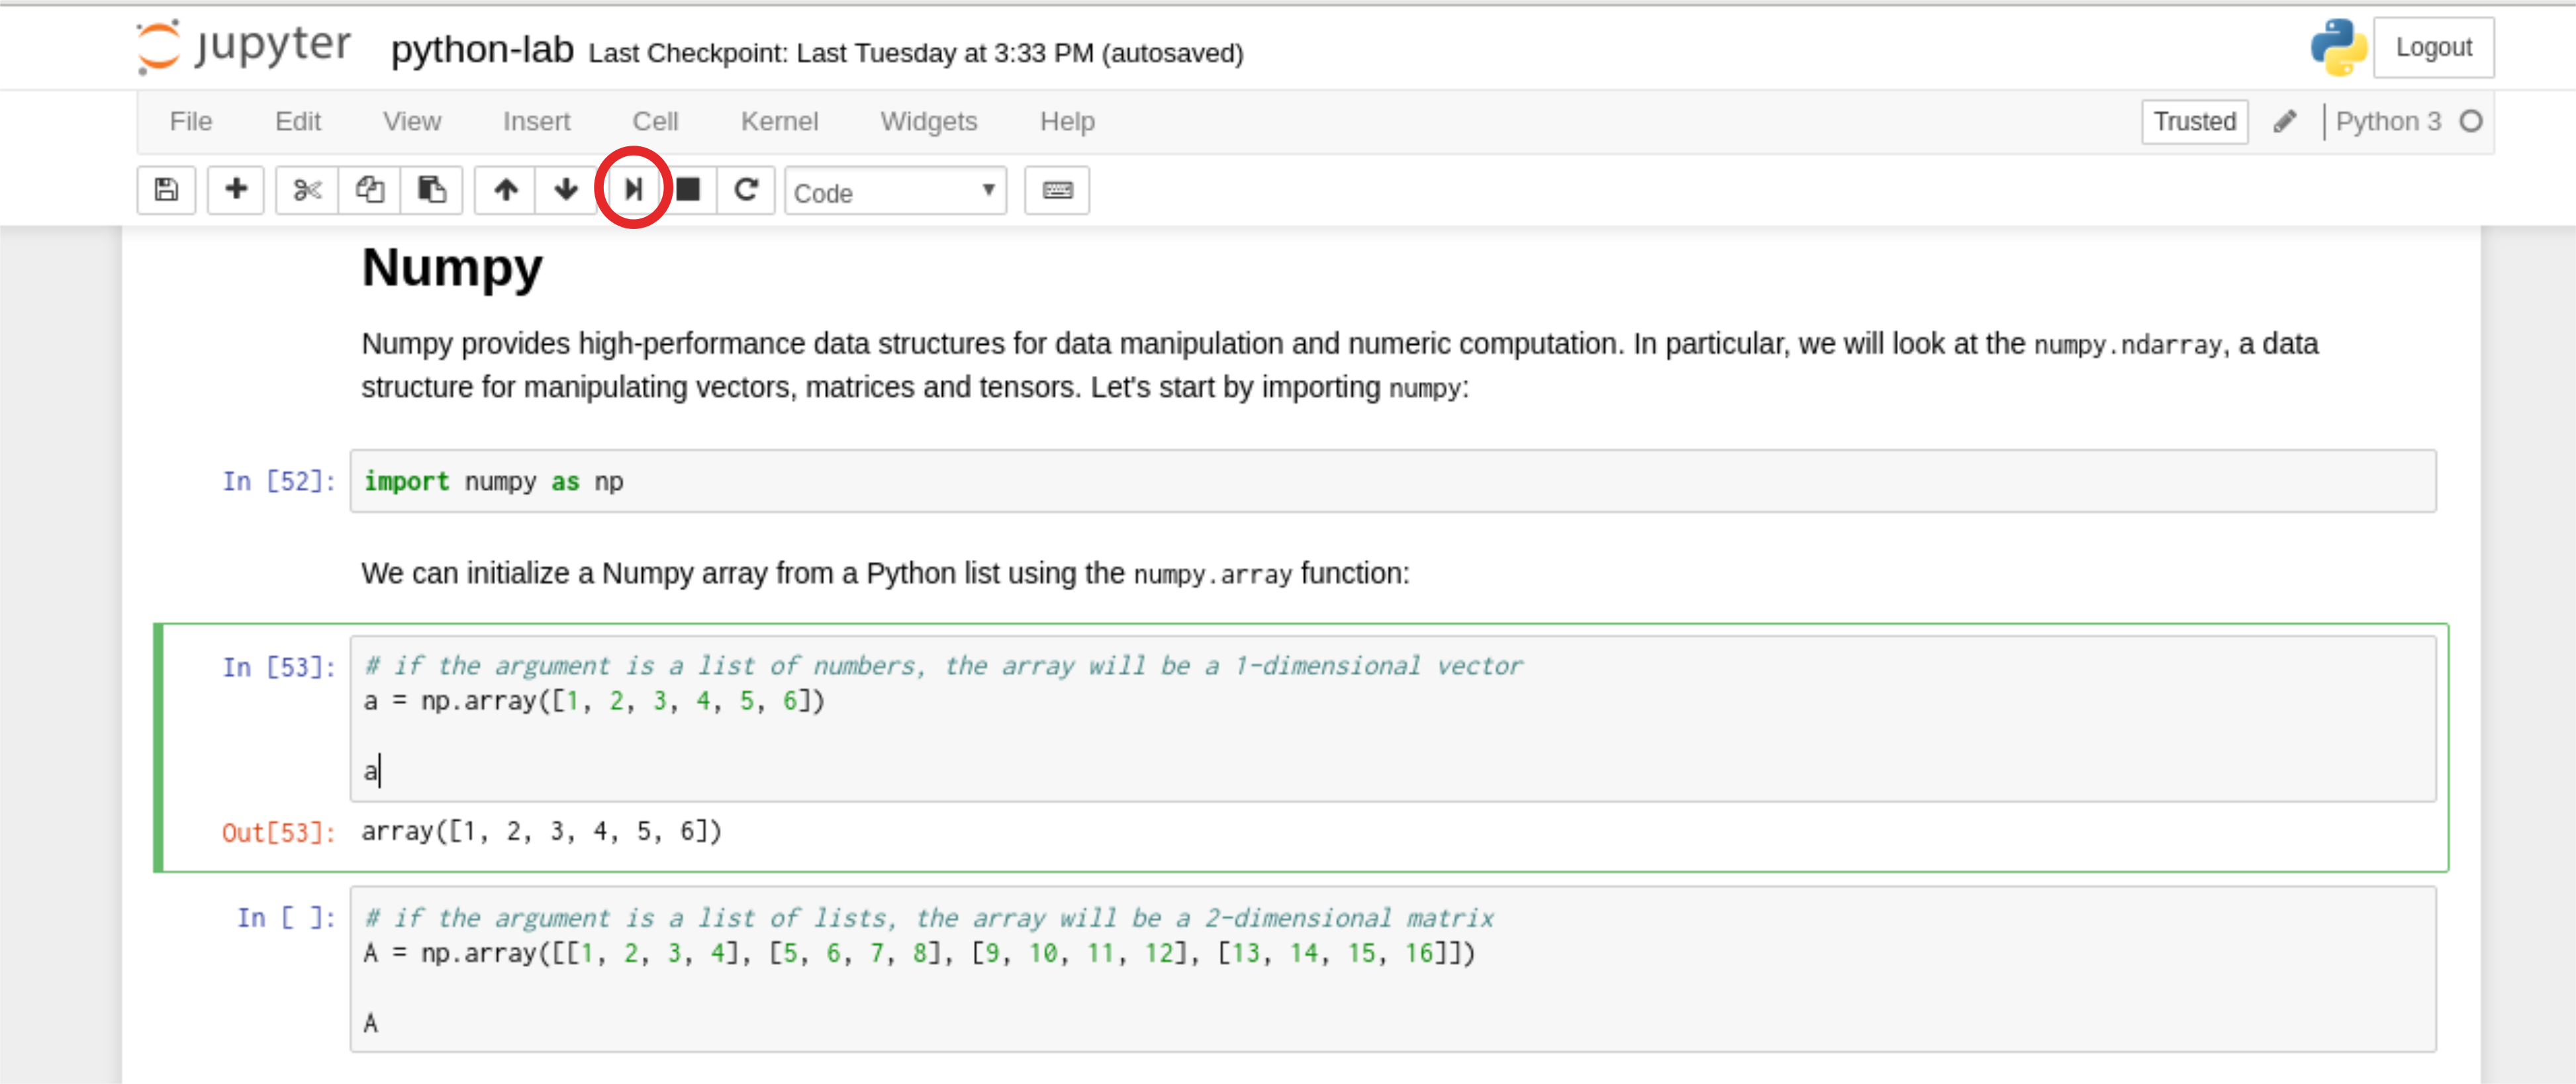
\includegraphics[width=\textwidth]{figures/click1}

\vspace{0.1in}
\hrule
\vspace{0.1in}

Execute commands by selecting a cell and clicking the \textcolor{tomato}{Run
button} on the header of the page or by \textbf{Shift+Enter}. You will see the
output of the command just below the cell.

You can tweak and modify the code as you wish and execute it again.

\end{frame}

%-----------------------------------------------------------------------------%

\begin{frame}{Assignment}
\centering

For the third Machine Learning assignment you will solve a classification task
using \textbf{TensorFlow} over the OCR dataset. The dataset is already split
into training and test sets. Your task is to train a deep
neural network on the training set and predict the labels on the test set. To
pass the assignment, your network has to classify the examples in the test
set with higher accuracy than the reference baseline for the dataset.

Additionally, you need to test your algorithm via cross-validation over the
training set and produce a report containing the results obtained.

\end{frame}

%-----------------------------------------------------------------------------%

\begin{frame}{Assignment | Material}

Download the assignment material:

{\footnotesize \url{http://disi.unitn.it/~passerini/teaching/2018-2019/MachineLearning/}}

The material motains:
    \begin{itemize}
    \item The training set examples;
    \item The training set labels;
    \item The test set examples;
    \item The test set labels;
    \item A README containing info about the dataset. \\ this file also contains
          the reference baseline accuracy;
    \end{itemize}

\end{frame}

%-----------------------------------------------------------------------------%

%\begin{frame}{Assignment | Helper}
%
%The helper script can be used to test your predictions. Given a file containing
%the predicted labels, the helper script sends the labels to our server and
%receives the prediction accuracy. You can use it in this way:
%
%\mint[fontsize=\scriptsize, bgcolor=GGrey]{cucumber}| >> ./helper.py your.email test-labels.txt |
%
%\vspace{-0.3in}
%The first parameter is your \texttt{unitn} email, the second parameter is the
%path to the file containing the predicted labels. This file should contain one
%label per line in the same order of the file containing the examples. The labels
%should be in the same format of the labels in the training set.
%
%The helper also prints the current best accuracy achieved by any of you on that
%dataset, just to put a bit of healthy competition! :)
%
%\end{frame}

%-----------------------------------------------------------------------------%

\begin{frame}{Assignment | Step-by-step}

\begin{enumerate}
\item Experiment with a deep network architecture of your choosing;
\item Test your network using cross-validation over the training set;
\item Train your classifier over the full training set;
\item Use the classifier to predict the examples in the test set;
\item Place the labels in a file, in the same order as you read the test
      examples and in the same format of the labels in the training set.
\item Write a report describing the learning algorithm used and discussing the
results obtained; The report should contain at least:
    \begin{itemize}
    \item The average accuracy over the folds and over the test set.
    \item A simple diagram of the network architecture (use Google Drawings or similar software);
    \end{itemize}
\end{enumerate}

\end{frame}

%-----------------------------------------------------------------------------%

\begin{frame}{Assignment | Submit}

\begin{itemize}
    \item After completing the assignment submit it via email
    \item Send an email to \href{mailto:mllab@unitn.it}{mllab@unitn.it} 
    \item Subject: tensorflowSubmit2018
    \item Attachment: \texttt{id\_name\_surname.zip} containing:
    \begin{itemize}
        \item The text file containing the final predictions;
        \item The code used to produce the predictions;
        \item The report in PDF format.
    \end{itemize}
\end{itemize}
\begin{alertblock}{NOTE}
    \begin{itemize}
	\item \textbf{No group work}
        \item This assignment is mandatory in order to enroll to the oral exam
    \end{itemize}
\end{alertblock}

\end{frame}

%-----------------------------------------------------------------------------%

\end{document}
